\documentclass[12pt,a4paper]{article}

\usepackage[T1]{fontenc}
\usepackage{amsmath, amssymb, amsfonts}
\usepackage[magyar]{babel}
\usepackage[utf8]{inputenc}
\usepackage{graphicx}
\usepackage{graphics}
\usepackage{mathtools}
\usepackage{epsfig}
\usepackage{epstopdf}
\usepackage{cite}
\usepackage{caption}
%\usepackage{hyperref}
\usepackage[bottom=4cm]{geometry}
%\geometry{a4paper, portrait, margin=1in}

\title{\huge{Korszerű vizsgálati módszerek labor jegyzőkönyv}\\ \vspace{20pt}
\textbf{Reaktorüzemeltetési gyakorlat} \\}

\author{\Large{\textsc{Csörnyei Géza}} \vspace{10pt}\\
	\textrm{Eötvös Loránd Tudományegyetem}\\
	\textrm{Fizika BSc III. évfolyam}
	}
\date{}
%\lhead{}
\begin{document}
\addtolength{\voffset}{-1.5cm}
\addtolength{\textheight}{1.5cm}
\begin{titlepage}
\maketitle

\begin{figure}[!htb]
\centering
  
\includegraphics[scale=0.6]{eltecimer.jpg}
\end{figure}

\hfil \Large{'C' mérőcsoport}\hfil  \\
\vspace*{2pt}
\hfil \Large{\emph{Mérés dátuma:} 2018.03.01.}\hfil \\
\vspace*{2pt}
\hfil \hspace*{45pt} \Large{\emph{Mérés vezetője:} Tormási Attila}\hfil
\thispagestyle{empty}
\end{titlepage}

\section{Bevezetés}
\hspace*{10pt} A mérés során megismerkedtünk a BME Oktatóreaktorának felépítésével és működésével, lehetőségünk nyílt a reaktor irányítására. Az instruktor által megadott, általunk beállított különböző reaktorteljesítmény értékek esetére megvizsgáltuk a szabályzó rudak kritikus működéshez szükséges helyzetét, majd megmértük a forrás eltávolítása után a reaktor értékességét különböző rúd pozíciók és teljesítményértékek esetére.

\section{Rövid elméleti összefoglaló}
\hspace*{10pt} Atomreaktornak nevezzük azon létesítményeket, melyekben az önfenntartó láncreakció külső forrás nélkül megvalósítható. A BME Oktatóreaktora egy termikus reaktor, mely azt jelenti, hogy benne a maghasadások döntő részét termikus neutronok hozzák létre. A reaktorok legfőbb részei: hasadóanyagot tartalmazó üzemanyag, a neutronok lassítására szolgáló moderátor,   a hűtőközeg és a működéshez, valamint a szabályozáshoz szükséges irányító rendszer.\\ 
\hspace*{10pt} Egy reaktort kritikus állapotúnak nevezünk, ha benne a láncreakció külső neutronforrás nélkül éppen megvalósul. A reaktorokat leíró legfontosabb mennyiség a neutronciklusonként történő neutronszám sokszorozódás értéke, az ún. effektív sokszorozódási tényező: 
\begin{equation}
k_{eff}=\epsilon \cdot p \cdot f \cdot \eta \cdot P,
\end{equation}
melyben az egyes faktorok sorrendben:
gyorshasítási tényező, rezonancia tényező, termikus hasznosítási tényező, termikus neutronhozam és a reaktor véges méretét figyelembe vevő kilépési tényező. Az így definiált tényező felhasználásával akkor mondunk kritikusnak egy reaktort, ha $k_{eff}=1$, azaz ha a reaktor teljesítménye időben állandó. Ha a tényező értéke kisebb vagy nagyobb mint 1, akkor ennek megfelelően a reaktor szub- vagy szuperkritikus.\\
\hspace*{10pt} Az effektív neutronsokszorozódási tényező segítségével definiálhatjuk a reaktor reaktivitását, az alábbi módon:
\begin{equation}
\rho=\frac{k_{eff}-1}{k_{eff}}
\end{equation}
A fentiek figyelembevételével $\rho=0$ jelenti a reaktor kritikusságát, $\rho<0$ jelenti a szubkritikusságot, $\rho>0$ pedig a szuperkritikusságot. A reaktorokban azonban nem csak közvetlenül a hasadásokból származó neutronok a fontosak, meghatározó szerepük van a hasadványmagok béta bomlásából származó ún. késő neutronoknak is. Ezek megjelenését a hasadványmagok bomlási ideje határozza meg, emiatt a hasadás után akár 1 perccel jelennek csak meg. Ezen neutronok részarányát jelöljük $\beta _{eff}$-el. Ha egy reaktor reaktivitása megegyezik ezen részaránnyal, akkor a reaktort promtkritikusnak nevezzük. Amennyiben ennél nagyobb a reaktivitás, az esetben a reaktor önmagát gerjesztheti, ezáltal szabályozhatatlanná válna, ha nem lennének negatív visszacsatolások.\\
\hspace*{10pt} Látható, hogy a reaktorban lejátszódó folyamatot, a $\frac{\rho}{\beta_{eff}}$ értéke határozza meg, ezt a hányadost nevezzük értékességnek. Mértékegysége: \$ . 

\section{Mérés menete}
\subsection{Kritikusság vizsgálata}
\hspace*{10pt} A mérés megkezdéséhez először a kezelő elektronika segítségével bejuttattuk a forrást az aktív térbe, majd kiemeltük a biztonsági rudakat, melyek a reaktor gyors leállítására szolgálnak. Ezt követően megemeltük a kézi és az automatikus szabályozó rudak helyzetét, hogy a teljesítmény elkezdjen nőni, egészen egy meghatározott értékig, amelynek elérésekor automatizáltra állítottuk a rendszert, így az magától beállította úgy a két rudat, hogy a reaktor kritikus legyen ilyen teljesítmény mellett. Először 1 W teljesítményre állítottuk a reaktort. Ekkor a két rúd helyzete:
\begin{table}[!h]
\begin{center}
\begin{tabular}{|c|c|}
\hline
Rúd & Kiemeltség (mm) \\
\hline
\hline
Automata & 429 \\
\hline
Kézi & 400 \\
\hline
\end{tabular}
\caption{A rudak helyzete (kiemeltsége) kritikus reaktor esetén (1 W)}
\end{center}
\end{table}

\hspace*{10pt} Következő lépésként kiemeltük a forrást az aktív térből, ezzel azonban, mivel a reaktor eleve kritikus volt, nem szakítottuk meg a láncreakciót. A forrás kiemelése után leolvastuk a rudak helyzetét:

\begin{table}[!h]
\begin{center}
\begin{tabular}{|c|c|}
\hline
Rúd & Kiemeltség (mm) \\
\hline
\hline
Automata & 436 \\
\hline
Kézi & 400 \\
\hline
\end{tabular}
\caption{A rudak helyzete (kiemeltsége) kritikus reaktor esetén (forrás nélkül)}
\end{center}
\end{table}

\hspace*{10pt} Az adatokból láthatóan az automatizált rúd helyzete megváltozott: ez annak köszönhető, hogy a korábbi esetben a reaktor kritikusságának fenntartásához nem csak láncreakciót, de a forrást is szabályozni kellett; utóbbi kiemelésével viszont lecsökkent a neutronfluxus, emiatt kicsit jobban ki kellett emelni az automata szabályzó rudat, hogy kritikus legyen a reaktor (máskülönben szubkritikussá vált volna). \\
\newpage
\subsection{Értékesség mérése}
\hspace*{10pt} A mérés következő lépése a reaktivitás meghatározása volt különböző szabályzórúd helyzetek esetére. Ezt a gamma kompenzált egyenáramú ionizációs kamra által mért beütésszám változásának sebességével tudtuk számolni: kiválasztottunk egy beütésszám tartományt, majd a reaktor kritikus helyzetből történő kimozdítása (az automata szabályzó rúd elmozdítása) után mértük mennyi idő alatt járjuk be ezt a tartományt. A mérést két különböző szabályzórúd állásból kiindulva végeztük el. A mérés során a reaktor teljesítménye 100 W volt.\\
A mérési eredmények az alábbiak:
\begin{table}[!h]
\begin{center}
\begin{tabular}{|c|c|c|}
\hline
- & 1. mérés & 2. mérés\\
\hline
Kézi sz. rúd helyzete (mm) & 460 & 400\\
\hline
Automata sz. rúd eltolt helyzete (mm) & 364 & 471 \\
\hline
Mért idő (s) & 53 & 127  \\
\hline
Számolt reaktivitás (cent) & 11.95 & 5.97 \\
\hline
\end{tabular}
\caption{Reaktivitás meghatározása 10 W teljesítményen}
\end{center}
\end{table} 
\newline
\hspace*{10pt} A beütésszám növekedése a szabályzó rúd kimozdításával volt kapcsolatban: azzal, hogy kijjebb helyeztük, szuperkritikus állapotba került a reaktor mindkét esetben. Az automata rudat mindig ugyanannyival mozdítottuk ki, a mérések között az egyetlen különbség a különböző kiindulási rúd helyzetek voltak. A reaktivitásokat a mérőhelyen, az ott kapott táblázat segítségévvel határoztuk meg. A tapasztalt reaktivitásbeli különbség a rúd jelleggörbéjével van kapcsolatban: minél messzebb van a szabályzó rúd, annál kevésbé lesz érzékeny rá a reaktorban lejátszódó folyamat, a jelleggörbén az integrált útkülönbség egyre kisebb lesz, azonos magasságkülönbség esetén. Emiatt mértünk jóval kisebb reaktivitást a második mérés során.\\
\newpage
\subsection{Doppler-visszacsatolás vizsgálata}
\hspace*{10pt} A laborgyakorlat során sikeresen felleltük a Doppler-visszacsatolás hatását is. Jelenség az üzemanyag hőmérsékletével van szoros kapcsolatban: magasabb hőmérsékleten a $^{238}$U rezonanciacsúcsai kiszélesednek, több neutron képes elnyelődni, ez a neutronfluxus csökkenéséhez vezet. A jelenség vizsgálatához 10 kW teljesítményen is meghatároztuk a kritikussághoz tartozó rúd helyzeteket úgy, hogy a kézi szabályzórúd helyzete megegyezzen azzal, mint amit 10 W esetén állítottunk. A kapott értékek:
\begin{table}[!h]
\begin{center}
\begin{tabular}{|c|c|}
\hline
Teljesítmény & Automata sz. rúd helyzete (mm)\\
\hline
10 W & 436 \\
\hline
10 kW & 483 \\
\hline
\end{tabular}
\caption{Doppler-visszacsatolás vizsgálata}
\end{center}
\end{table}
\newline
A kapott értékek alapján valóban kisebb volt a neutronfluxus, emiatt kellett kijjebb helyezni a automata szabályzó rudat. Következésképpen a hőmérséklet növekedése esetén valóban lecsökken a neutronfluxus.\\
\newpage
\subsection{Ionizációs kamrák vizsgálata}
\hspace*{10pt} A méréssorozat utolsó lépéseként megvizsgáltuk a hasadási és a gamma kompenzált egyenáramú ionizációs kamrák által mért beütésszámok teljesítményfüggését. A kapott beütésszámok különböző teljesítményekhez tartozó kritikus állapotok esetére (a kamrák típusát kezdetben nem ismertük):
\begin{table}[!h]
\begin{center}
\begin{tabular}{|c|c|c|}
\hline
Teljesítmény & 1. kamra beütésszám & 2. kamra beütésszám\\
\hline
\hline
10 W & $1\cdot 10^4$ & $0.22\cdot 10^5$\\
\hline
100 W & $1.2 \cdot 10^5 $ & $0.22\cdot 10^6$ \\
\hline
200 W & $2.2 \cdot 10^5 $ & $0.44 \cdot 10^6$ \\
\hline
1 kW & $1.2 \cdot 10^6 $ & $1.2 \cdot 10^6 $\\
\hline
2 kW & $2.5\cdot 10^6 $ & $1.7\cdot 10^6$ \\
\hline
\end{tabular}
\caption{Beütésszámok teljesítményfüggése}
\end{center}
\end{table}
\newline
A fenti értékeket ábrázolhatjuk és vizsgálhatjuk a linearitástól vett eltéréseket. Erre azért van szükség, mert ezzel megkülönböztethető a két detektor: míg a beütésszám a teljesítménnyel egyenes arányban növekszik, melyet a gamma kompenzált ionizációs kamra le is tud követni, addig a hasadási kamrákra ez csak kis teljesítmények esetén igaz, nagyobb teljesítmények esetén ezen kamra nemlineáris függést mutat, majd telítésbe megy. A készített ábrák:
\begin{figure}[!h]
\centering
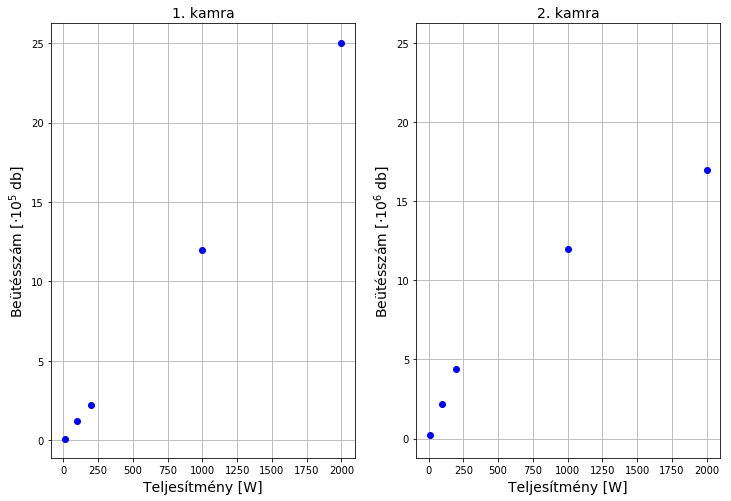
\includegraphics[scale=0.5]{Kamrak.png}
\caption{A két kamra által mért beütésszámok teljesítményfüggése}
\end{figure}
\newline
Az ábrák alapján biztosan kijelenthető, hogy a 2. kamra volt a hasadási ionizációs kamra, ugyanis a teljesítményfüggés jól láthatóan elveszíti lineáris jellegét a másik kamrával ellentétben.\\

\section{Diszkusszió}
\hspace*{10pt} A laborgyakorlat során elsajátítottuk a BME Oktatóreaktorának kezelésének alapjait, megvizsgáltuk a kritikussághoz szükséges szabályzó rúd helyzetek neutronfluxus-függését, meghatároztuk a reaktivitást két különböző állapotból kiindulva, kimutattuk a Dopplet-visszacsatolás jelenségét, valamint ellenőriztük a neutronfluxus mérésére használt ionizációs kamrák beütésszámának teljesítményfüggését.

\end{document}